%% LyX 2.0.3 created this file.  For more info, see http://www.lyx.org/.
%% Do not edit unless you really know what you are doing.
\documentclass[english]{article}
\usepackage[T1]{fontenc}
\usepackage[latin9]{inputenc}
\usepackage{float}
\usepackage{graphicx}
\usepackage{babel}
\begin{document}

\section{Introducere}

DataBrowser este componentul central al interfetei publice RODA. Prin
intermediul acestuia, utilizatorii vor interactiona cu baza de date
de studii, vor cauta datele care ii intereseaza si vor putea accesa
datele identificate, in functie de drepturile pe care le au. 

DataBrowser-ul va evolua pe toata durata dezvoltarii sistemului RODA,
odata cu adaugarea noilor carac- teristici pe care le presupune procesul
de dezvoltare. In aceasta faza, componentul permite ordonarea studiilor
dupa ani sau cataloage si vizualizarea datelor fiecarui studiu in
parte. 

DataBrowserul este o interfata dinamica construita cu ajutorul urmatoarelor
principii si tehnologii: Intreaga interfata este scrisa in limbajul
Javascript utilizand setul de librarii Ext Js. Ext JS este un set
complet de instrumente special proiectat pentru programarea aplicatiilor
dinamice care ruleaza in programele de navigare pe internet. Astfel,
interfata DataBrowser este un program client care comunica cu serverul
cu ajutorul apelurilor HTTP si primeste date in format JSON (JavaScript
Object Notation)

\begin{figure}[H]
\begin{centering}
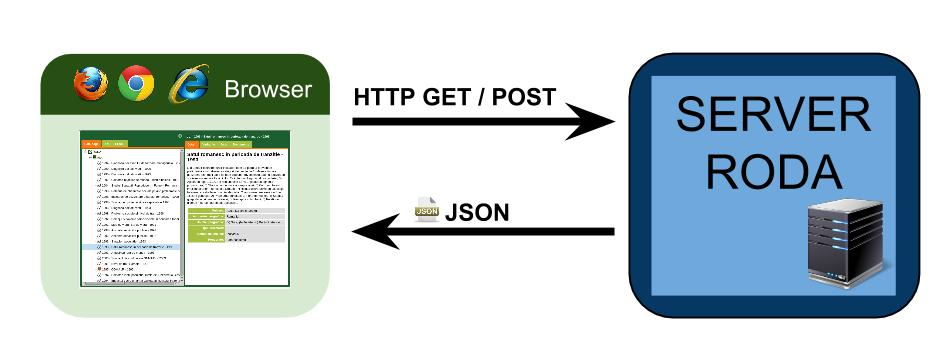
\includegraphics[width=9cm]{img/db-server}
\par\end{centering}

\caption{Modul simplificat de comunicare intre databrowser si server}
\end{figure}

\section{Controller-e JSON pe partea de server}


Controller-ele care stau la baza componentei Data Browser a aplicatiei utilizeaza servicii care, la randul lor, refera anumite clase speciale din domeniu. Aceste clase extind o clasa de baza (\emph{JsonInfo}), ce contine atributele comune ale claselor utilizate pentru obtinerea rezultatelor in format JSON. Pe langa acestea, atributul \emph{type} al clasei permite distinctia intre obiectele de diferite tipuri ce apar in ierarhii. Astfel, vom avea elemente al caror tip este M (nod principal, radacina in cazul ierarhiilor), C (catalog), S (serie), St (studiu), Sts (studiu ce provine dintr-o serie), Y (an).  
Subclasele lui \emph{JsonInfo} structureaza informatia necesara in rezultatul controller-elor, furnizand metode statice de generare a colectiilor corespunzatoare sau a obiectelor identificate cu ajutorul valorii cheii primare sau a altor campuri (de exemplu, valoarea anului pentru ierarhia de ani si studii). Cu ajutorul acestor metode, clasele ce extind \emph{JsonInfo} permit obtinerea de informatii complexe, care vizeaza mai multe clase ale domeniului de baza al aplicatiei.
Transformarea colectiilor sau obiectelor in format JSON s-a efectuat cu ajutorul bibliotecii \emph{Flexjson} (\url{http://flexjson.sourceforge.net/}) care permite serializarea, respectiv deserializarea obiectelor Java in si din JSON.  

Ierarhia de clase ce deriva din \emph{JsonInfo} cuprinde urmatoarele clase:
\begin{itemize}
\item
\emph{CatalogTree} - genereaza arborescenta de cataloage, pornind de la un nod principal (M), urmat de cataloagele radacina (care nu au un catalog parinte). La nivelul fiecarui catalog este indicat tipul acestuia (C sau S), iar la nivelul fiecarui studiu este indicat tipul acestuia (St sau Sts). Un studiu poate apartine si unui alt catalog, de tip serie; astfel, in cazul unui studiu de tip Sts este indicat si codul seriei care il contine. In frunzele arborelui se afla studiile.
\item
\emph{StudiesByCatalog} - prezinta studiile din cadrul fiecarui catalog din baza de date. La nivelul fiecarui catalog este indicat numarul studiilor sale, iar la nivelul fiecarui studiu este indicat tipul acestuia (St sau Sts). 
\item
\emph{StudiesBySeries} - prezinta studiile din seriile din baza de date; pentru fiecare serie, este specificat si numarul studiilor din cadrul sau. 
\item
\emph{StudiesByTopic} - prezinta studiile corespunzatoare fiecarui topic.
\item
\emph{StudiesByYear} - prezinta studiile corespunzatoare fiecarui an in care s-au realizat studii, precum si numarul acestora. La nivelul fiecarui studiu este specificat tipul (St sau Sts).
\item
\emph{StudyInfo} - genereaza informatii complete despre studiile din baza de date, incluzand variabilele, persoanele, organizatiile, fisierele si cuvintele cheie asociate) 
\item
\emph{YearsTree} - genereaza ierarhia corespunzatoare anilor, pornind de la un nod principal (M), ai carui fii (de tip Y) corespund anilor de realizare a studiilor din baza de date. La nivelul fiecarui studiu este indicat tipul acestuia (St sau Sts) 
\end{itemize}

Fiecarei clase de mai sus ii corespunde un controller (\emph{<nume_clasa>Controller}), ce utilizeaza un serviciu asociat (\emph{<nume_clasa>Service}).


\section{API}

In acest moment, interfata serverului pentru databrowser contine urmatoarele
apeluri si rezultate:


\subsection{CatalogTree}

Returneaza o lista a tuturor cataloagelor generale din sistem impreuna
cu studiile asociate acestora. Structura este arborescenta, elementul
de container se numeste \textquotedbl{}data\textquotedbl{}

\begin{figure}[H]
\begin{centering}
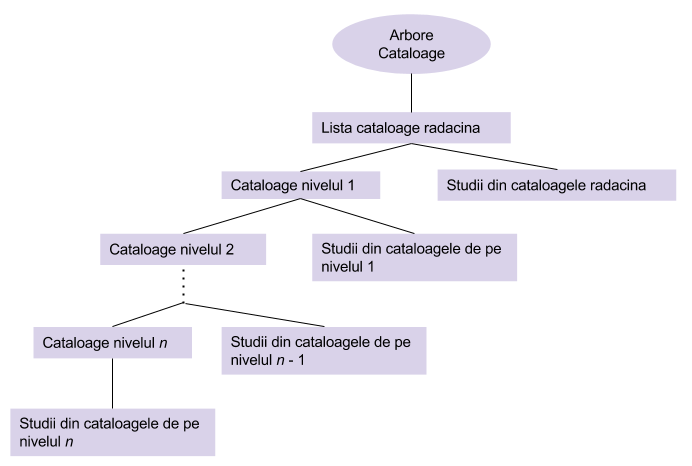
\includegraphics[width=9cm]{img/catalogtree}
\par\end{centering}

\caption{Etapele de procesare ale serverului necesare pentru returnarea raspunsului}


\end{figure}

\begin{itemize}
\item \textbf{name} - Numele catalogului 
\item \textbf{type} - Tipul catalogului 

\begin{itemize}
\item \textbf{M} - Master catalog, catalogul principal, radacina pentru
celelalte cataloage publice 
\item \textbf{C} - Catalog normal 
\item \textbf{S} - Serie (studii grupate de catre executanti dupa orice
criteriu) 
\end{itemize}
\item \textbf{indice} - indexul numeric unic al catalogului din baza de
date 
\item \textbf{data} - continutul catalogului. Acesta poate cuprinde alte
cataloage (cu aceeasi structura ca mai sus), serii sau studii 

\begin{itemize}
\item \textbf{an} - Anul in care a fost finalizat studiul 
\item \textbf{description} - rezumatul studiului 
\item \textbf{geographicUnit} - Unitatea geografica pe care se bazeaza realizarea
studiului 
\item \textbf{indice} - id-ul unic din baza de date al studiului 
\item \textbf{name} - titlul studiului 
\item \textbf{researchInstrument }- Tipul cercetarii 
\item \textbf{seriesId} - in cazul in care studiul este membru al unei serii,
aici se inregistreaza, pentru referinta, id-ul unic din baza de date
al seriei respective 
\item \textbf{type} - tipul studiului, care determina mudul de afisare in
panoul de detalii 

\begin{itemize}
\item \textbf{St} - studiu izolat 
\item \textbf{Sts} - membru al unei serii weighting - metoda de ponderare
folosita
\end{itemize}
\end{itemize}
\end{itemize}

\subsection{YearTree}

Returneaza o lista a tuturor anilor din sistem care au studii asociate
acestora, impreuna cu studiile corespunzatoare. Structura este arborescenta,
elementul de container se numeste \textquotedbl{}data\textquotedbl{}.
Structura este deschisa de un nod unic principal.

\begin{figure}[H]
\begin{centering}
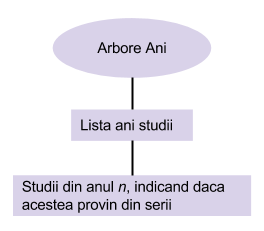
\includegraphics[width=4cm]{img/yearstree}
\par\end{centering}

\caption{Etapele de procesare ale serverului}


\end{figure}



\paragraph{Nodul principal}
\begin{itemize}
\item \textbf{name} - Numele nodului principal (doar in cazul nodului principal) 
\item \textbf{type} - Tipul nodului 
\item \textbf{M }- Master, nodul principal, radacina pentru nodurile pe
ani 
\item \textbf{data} - continutul nodului (lista nearborescenta de ani)
\end{itemize}

\paragraph{Nod de tip an}
\begin{itemize}
\item \textbf{name} - Numele nodului de tip an 
\item \textbf{an} - Anul nodului curent 
\item \textbf{type} - Y 
\item \textbf{data} - continutul nodului (lista nearborescenta de studii) 

\begin{itemize}
\item \textbf{an} - Anul in care a fost finalizat studiul 
\item \textbf{description} - rezumatul studiului 
\item \textbf{geographicUnit} - Unitatea geografica pe care se bazeaza realizarea
studiului 
\item \textbf{indice} - id-ul unic din baza de date al studiului 
\item \textbf{name} - titlul studiului 
\item \textbf{researchInstrument} - Tipul cercetarii 
\item \textbf{seriesId} - in cazul in care studiul este membru al unei serii,
aici se inregistreaza, pentru referinta, id-ul unic din baza de date
al seriei respective 
\item \textbf{type} - tipul studiului, care determina mudul de afisare in
panoul de detalii 

\begin{itemize}
\item \textbf{St} - studiu izolat 
\item \textbf{Sts} - membru al unei serii 
\end{itemize}
\item \textbf{weighting} - metoda de ponderare folosita 
\end{itemize}
\end{itemize}

\subsection{StudyInfo}

Returneaza principalele componente ale structurii asociate unui studiu

\begin{figure}[H]
\begin{centering}
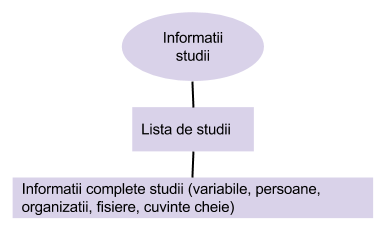
\includegraphics[width=5cm]{img/studyinfo}
\par\end{centering}

\caption{Etapele de procesare ale serverului necesare pentru returnarea raspunsului}


\end{figure}

\begin{itemize}
\item \textbf{an} - Anul in care a fost finalizat studiul 
\item \textbf{description} - rezumatul studiului 
\item \textbf{geographicUnit} - Unitatea geografica pe care se bazeaza realizarea
studiului 
\item \textbf{indice} - id-ul unic din baza de date al studiului 
\item \textbf{name} - titlul studiului 
\item \textbf{researchInstrument} - Tipul cercetarii 
\item \textbf{seriesId} - in cazul in care studiul este membru al unei serii,
aici se inregistreaza, pentru referinta, id-ul unic din baza de date
al seriei respective 
\item \textbf{type} - tipul studiului, care determina mudul de afisare in
panoul de detalii 

\begin{itemize}
\item \textbf{St} - studiu izolat 
\item \textbf{Sts} - membru al unei serii 
\end{itemize}
\item \textbf{weighting} - metoda de ponderare folosita 
\item \textbf{research\_instrument} - Tipul de cercetare 
\item \textbf{unit\_analysis} - Unitatea de analiza a studiului 
\item \textbf{universe} - universul studiului 
\item \textbf{keywords} - Cuvintele cheie ale studiului 
\item \textbf{orgs} - Organizatii asociate studiului 
\item \textbf{persons} - Persoane asociate studiului 
\item \textbf{variables} - Colectie de variabile 

\begin{itemize}
\item \textbf{nrfreq} - Numarul frecventelor calculate pentru variabila
curenta 
\item \textbf{indice} - Indexul unic al variabilei in baza de date 
\item \textbf{label }- Eticheta variabilei 
\item \textbf{name} - Numele variabilei 
\end{itemize}
\end{itemize}

\subsection{StudiesbyCatalog}

Returneaza un nod de tip catalog impreuna cu toate studiile care fac
parte din acel catalog, in lista aplatizata (daca exista subcataloage
acestea nu sunt returnate dar studiile asociate lor, da).

\begin{figure}[H]
\begin{centering}
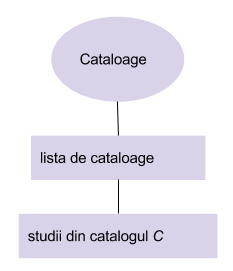
\includegraphics[width=4cm]{img/studiesbycatalog}
\par\end{centering}

\caption{Etapele de procesare ale serverului necesare pentru returnarea raspunsului}


\end{figure}

\begin{itemize}
\item \textbf{name} - Numele catalogului 
\item \textbf{nrstudies} - Numarul de studii 
\item \textbf{indice} - indexul numeric unic al catalogului din baza de
date 
\item \textbf{data} - continutul catalogului. Acesta cuprinde doar studii,
indiferent de structura arborescenta a subcataloagelor.

\begin{itemize}
\item \textbf{an} - Anul in care a fost finalizat studiul 
\item \textbf{description} - rezumatul studiului 
\item \textbf{geographicUnit} - Unitatea geografica pe care se bazeaza realizarea
studiului 
\item \textbf{indice} - id-ul unic din baza de date al studiului 
\item \textbf{name} - titlul studiului 
\item \textbf{researchInstrument} - Tipul cercetarii 
\item \textbf{seriesId} - in cazul in care studiul este membru al unei serii,
aici se inregistreaza, pentru referinta, id-ul unic din baza de date
al seriei respective 
\item \textbf{type} - tipul studiului, care determina modul de afisare in
panoul de detalii 

\begin{itemize}
\item \textbf{St} - studiu izolat 
\item \textbf{Sts }- membru al unei serii 
\end{itemize}
\item \textbf{weighting} - metoda de ponderare folosita 
\end{itemize}
\end{itemize}

\subsection{StudiesbySeries}

Returneaza un nod de tip serie impreuna cu toate studiile care fac
parte din aceasta

\begin{figure}[H]
\begin{centering}
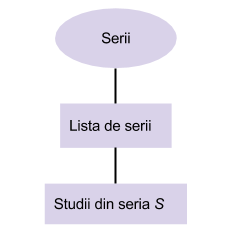
\includegraphics[width=4cm]{img/series}
\par\end{centering}

\caption{Etapele de procesare ale serverului necesare pentru returnarea raspunsului}


\end{figure}

\begin{itemize}
\item \textbf{description} - rezumatul seriei 
\item \textbf{geographicUnit} - Unitatea geografica pe care se bazeaza realizarea
seriei 
\item \textbf{indice} - id-ul unic din baza de date al seriei 
\item \textbf{name} - titlul seriei 
\item \textbf{researchInstrument} - Tipul cercetarii 
\item \textbf{weighting} - metoda de ponderare folosita, daca este comuna 
\item \textbf{research\_instrument} - Tipul de cercetare 
\item \textbf{unit\_analysis} - Unitatea de analiza a seriei 
\item \textbf{universe} - universul seriei 
\item \textbf{keywords} - Cuvintele cheie ale seriei 
\item \textbf{orgs }- Organizatii asociate seriei 
\item \textbf{persons} - Persoane asociate seriei 
\item \textbf{data} - continutul seriei, lista de studii 

\begin{itemize}
\item \textbf{an} - Anul in care a fost finalizat studiul 
\item \textbf{description} - rezumatul studiului 
\item \textbf{geographicUnit} - Unitatea geografica pe care se bazeaza realizarea
studiului 
\item \textbf{indice} - id-ul unic din baza de date al studiului 
\item \textbf{name} - titlul studiului 
\item \textbf{researchInstrument} - Tipul cercetarii 
\item \textbf{seriesId} - in cazul in care studiul este membru al unei serii,
aici se inregistreaza, pentru referinta, id-ul unic din baza de date
al seriei respective 
\item \textbf{type} - tipul studiului, care determina modul de afisare in
panoul de detalii 

\begin{itemize}
\item \textbf{Sts} - membru al unei serii 
\end{itemize}
\item \textbf{weighting} - metoda de ponderare folosita 
\end{itemize}
\end{itemize}

\subsection{StudiesbyYear}

Lista tuturor studiilor din acelasi an

Returneaza un nod principal de tip an impreuna cu toate studiile asociate
acestuia

\begin{figure}[H]
\begin{centering}
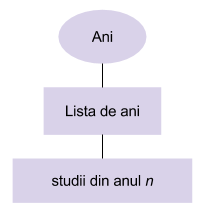
\includegraphics[width=4cm]{img/studiesbyyear}
\par\end{centering}

\caption{Etapele de procesare ale serverului necesare pentru returnarea raspunsului}


\end{figure}

\begin{itemize}
\item \textbf{name} - Numele nodului de tip an 
\item \textbf{an} - Anul nodului curent 
\item \textbf{type} - Y 
\item \textbf{data} - continutul nodului (lista nearborescenta de studii) 

\begin{itemize}
\item \textbf{an} - Anul in care a fost finalizat studiul 
\item \textbf{description} - rezumatul studiului 
\item \textbf{geographicUnit} - Unitatea geografica pe care se bazeaza realizarea
studiului 
\item \textbf{indice} - id-ul unic din baza de date al studiului name -
titlul studiului 
\item \textbf{researchInstrument} - Tipul cercetarii 
\item \textbf{seriesId} - in cazul in care studiul este membru al unei serii,
aici se inregistreaza, pentru referinta, id-ul unic din baza de date
al seriei respective 
\item \textbf{type} - tipul studiului, care determina modul de afisare in
panoul de detalii 

\begin{itemize}
\item \textbf{St} - studiu izolat 
\item \textbf{Sts} - membru al unei serii 
\end{itemize}
\item \textbf{weighting} - metoda de ponderare folosita
\end{itemize}
\end{itemize}

\section{Interfata}

Interfata DataBrowser-ului este compusa din doua zone principale,
zona de index si zona de detaliu. Zona de index contine mai multe
ecrane care afiseaza studiile aflate in baza de date in functie de
diferite criterii de grupare. Zona de index este construita pentru
a afisa diferite modalitati de trecere in revista a tuturor studiilor
din baza de date. In functie de necesitati, se pot adauga noi ecrane
care sa permita noi modalitati de grupare sau filtrare. Zona de detaliu
contine diferite tipuri de ecrane care afiseaza detalii despre elementul
selectat in zona de index. 

\begin{figure}[H]
\begin{centering}
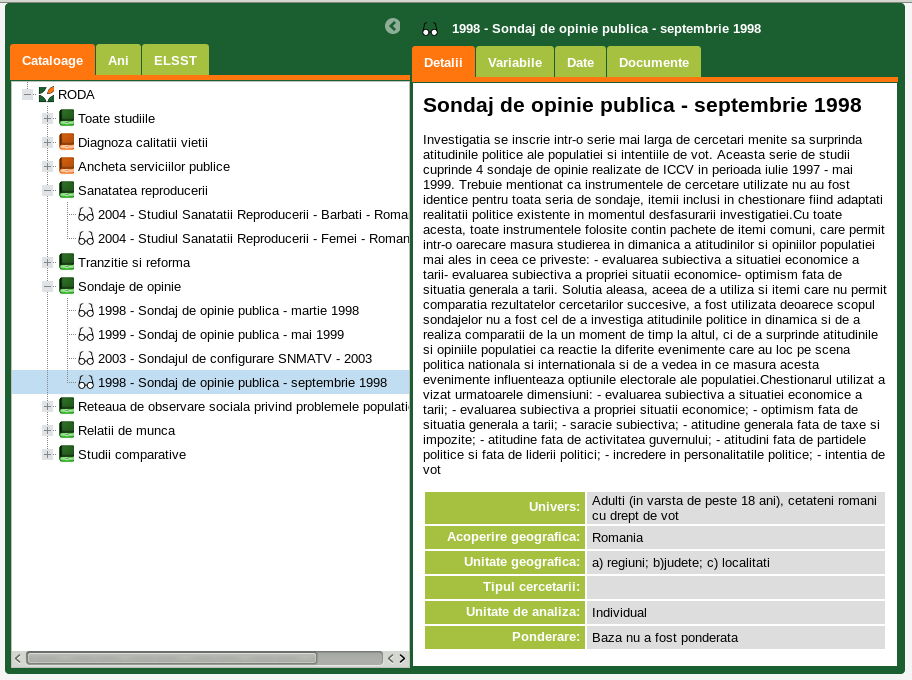
\includegraphics[width=11cm]{screenshots/databrowser-general}
\par\end{centering}

\caption{Databrowser}


\end{figure}



\subsection{Ecranele din zona de index}


\subsubsection{Cataloage}

Ecranul ``Cataloage'' afiseaza o structura arborescenta de cataloage,
serii si studii. Cataloagele sunt elemente arbitrare de grupare propuse
de RODA pentru gruparea studiilor. Cataloagele pot fi incluse in alte
cataloage. Un studiu poate fi membru in mai multe cataloage si in
acest caz el va aparea in toate. 

Un caz particular al cataloagelor sunt seriile. Seriile reprezinta
grupari ne-arbitrare de studii, alaturate conform unui criteriu important,
cum ar fi tematica lor. 

\begin{figure}[H]
\begin{centering}
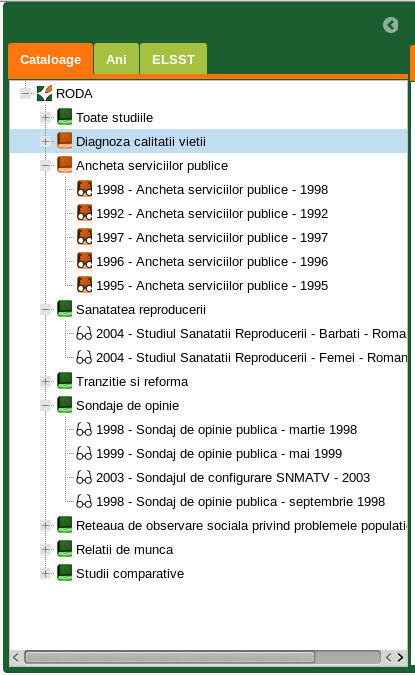
\includegraphics[width=6cm]{screenshots/left-panel-cataloage}
\par\end{centering}

\caption{Ecranul ``Cataloage''}
\end{figure}



\subsubsection{Ani}

Ecranul ``Ani'' afiseaza o structura arborescenta in care studiile
sunt grupate dupa ani. Studiile care sunt membre in serii sunt evidentiate.
Seriile ca elemente de sine statatoare nu pot aparea aici pentru ca
studiile din aceeasi serie pot fi (si de obicei sunt) finalizate in
ani diferiti. 

\begin{figure}[H]
\begin{centering}
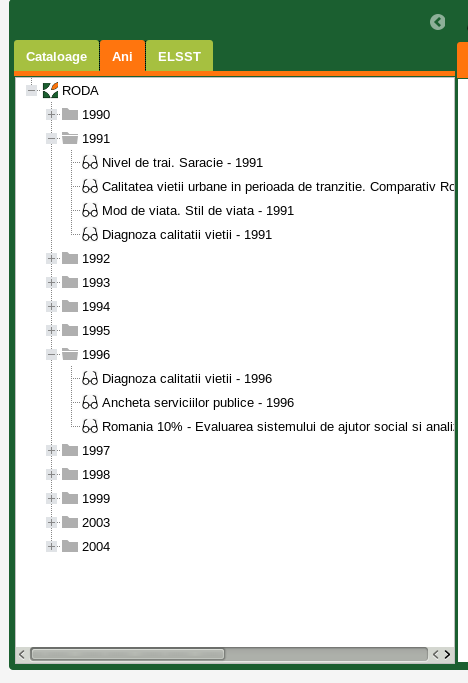
\includegraphics[width=6cm]{screenshots/left-panel-ani}
\par\end{centering}

\caption{Ecranul ``Ani''}


\end{figure}



\subsection{Ecrane din zona de detaliu}


\subsubsection{Catalog}

Ecranul pentru vizualizarea catalogului afiseaza toate studiile din
catalogul selectat. Acest ecran apare doar cand in zona de index se
selecteaza un element de tip catalog. Acesta contine elemente care
permit cautarea locala (in catalogul curent) precum si elemente de
paginare. Ecranul pentru vizualizarea catalogului poate avea trei
densitati de informatie diferite. In cele ce urmeaza vor fi prezentate
cele trei ecrane asa cum sunt ele acum. Trebuie mentionat insa ca
elementele din cele trei ecrane se pot modifica in functie de evaluarea
utilizabilitatii interfetei.

\begin{figure}[H]
\begin{centering}
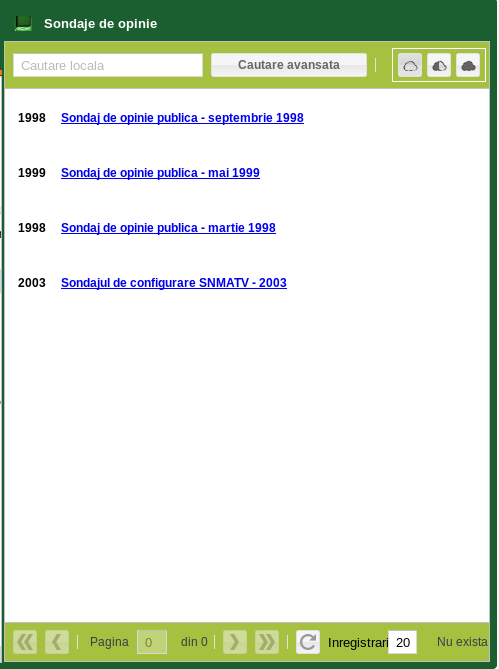
\includegraphics[width=6cm]{screenshots/details-panel-catalog-simple}
\par\end{centering}

\caption{Ecranul de tip Catalog - densitate de informatie mica}


\end{figure}


Ecranul cu densitate de informatie mica afiseaza anul si titlul studiului.
Titlul studiului este in acelasi timp si un link. La accesarea acestuia,
ecranul catalogului va fi inlocuit de ecranul care prezinta studiul
respectiv. 

\begin{figure}[H]
\begin{centering}
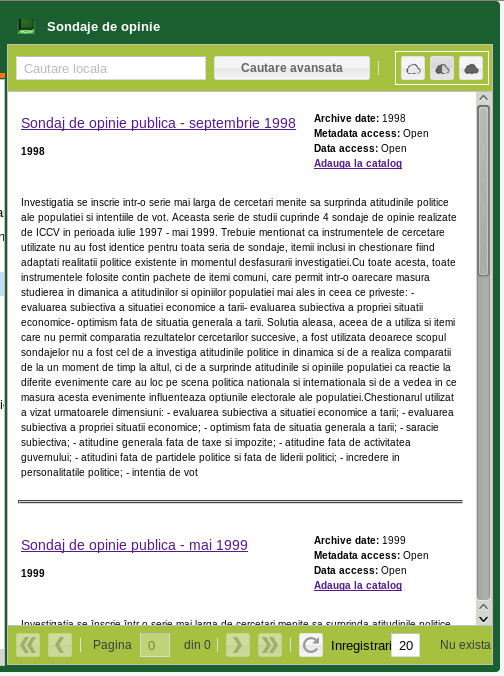
\includegraphics[width=6cm]{screenshots/details-panel-catalog-medium}
\par\end{centering}

\caption{Ecranul de tip Catalog - densitate de informatie medie}


\end{figure}


Ecranul cu densitate de informatie medie afiseaza titlul studiilor,
anul, informatii despre accesibilitatea metadatelor si datelor si
descrierea acestora. Pentru utilizatorii inregistrati va exista si
optiunea de a adauga studiile la un catalog personal. 

\begin{figure}[H]
\begin{centering}
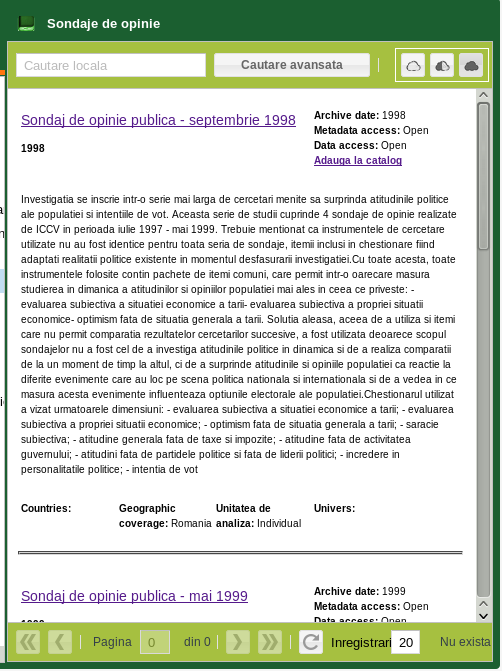
\includegraphics[width=6cm]{screenshots/details-panel-catalog-large}
\par\end{centering}

\caption{Ecranul de tip catalog - densitate de informatie mare}


\end{figure}


Ecranul cu densitate mare de informatie afiseaza toate informatiile
pe care le afiseaza ecranul cu densitate medie la care se adauga si
informatiile de localizare, unitatea de analiza, precum si alte elemente
tehnice care sunt dependente de tipul studiului. 


\subsection{Ani}

Ecranul pentru vizualizarea unui an afiseaza toate studiile din acel
an. Acest ecran apare doar cand in zona de index se selecteaza un
element de tip an. Ecranul contine elemente care permit cautarea locala
(in catalogul curent) precum si elemente de paginare. Ecranul pentru
vizualizarea anului poate avea trei densitati de informatie diferite. 

\begin{figure}[H]
\begin{centering}
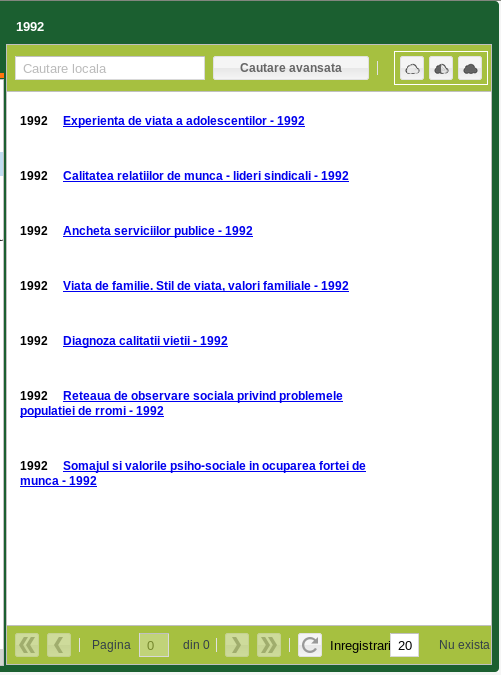
\includegraphics[width=6cm]{screenshots/details-panel-an-simple}
\par\end{centering}

\caption{Ecranul de tip an - densitate de informatie mica}


\end{figure}


Ecranul cu densitate de informatie mica afiseaza anul si titlul studiului.
Titlul studiului este in acelasi timp si un link. La accesarea acestuia,
ecranul catalogului va fi inlocuit de ecranul care prezinta studiul
respectiv. 

\begin{figure}[H]
\begin{centering}
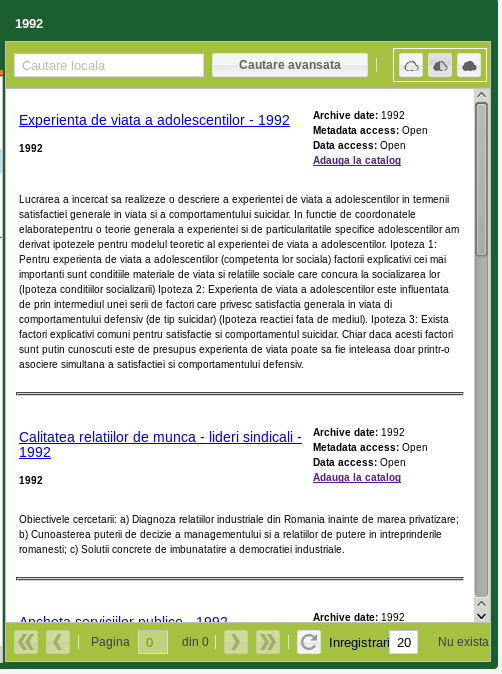
\includegraphics[width=6cm]{screenshots/details-panel-an-medium}
\par\end{centering}

\caption{Ecranul de tip an - densitate de informatie medie}


\end{figure}


Ecranul cu densitate de informatie medie afiseaza titlul studiilor,
anul, informatii despre accesibilitatea metadatelor si datelor si
descrierea acestora. Pentru utilizatorii inregistrati va exista si
optiunea de a adauga studiile la un catalog personal. 

\begin{figure}[H]
\begin{centering}
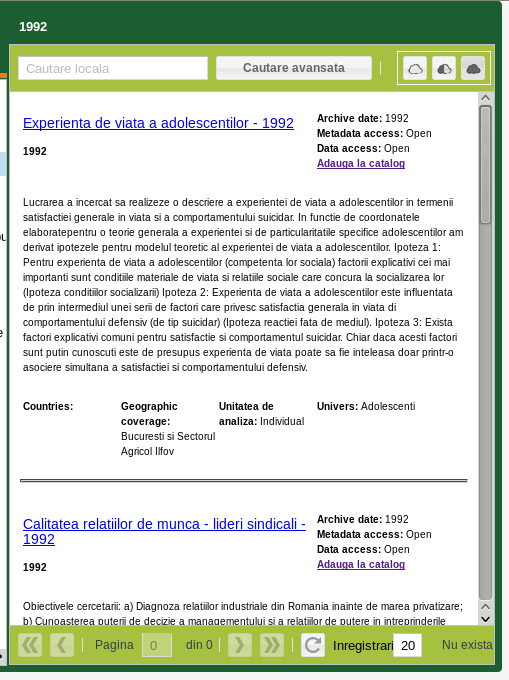
\includegraphics[width=6cm]{screenshots/details-panel-an-large}
\par\end{centering}

\caption{Ecranul de tip an - densitate de informatie mare}
\end{figure}


\pagebreak{}


\subsection{Studiu}

Ecranul pentru afisarea unui studiu contine in acest moment patru
sub-ecrane. Acestea sunt configurate pentru studii de tip chestionar,
acestea fiind cele disponibile pentru date de testare. Pe masura ce
apar alte tipuri de studii, cu alte tipuri de metadate si date, structura
ecranului de studii se va modifica. 

\begin{figure}[H]
\begin{centering}
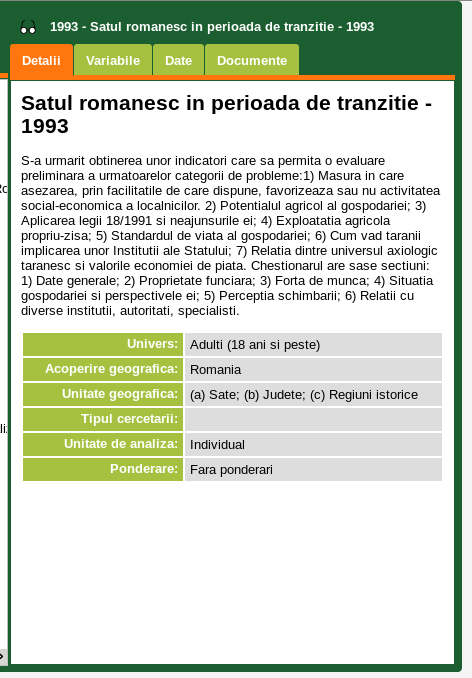
\includegraphics{screenshots/details-panel-study-detalii}
\par\end{centering}

\caption{Ecranul studiu, subecranul ``Detalii''}
\end{figure}


Subecranul ``detalii `` afiseaza titlul, descrierea si celelalte
metadate asociate studiului respectiv. In functie de metadatele disponibile
acest ecran poate contine diferite tipuri de informatii. Acest sub-ecran
va fi mentinut in toate ecranele care vor fi folosite pentru afisarea
diferitelor tipuri de studii.

\begin{figure}[H]
\begin{centering}
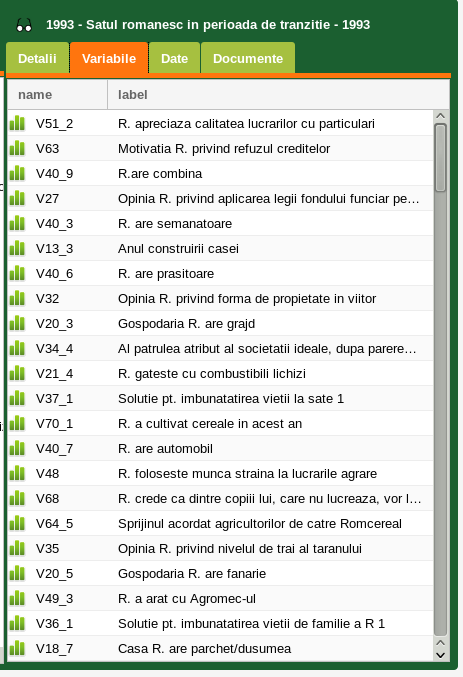
\includegraphics[width=6cm]{screenshots/details-panel-study-variabile}
\par\end{centering}

\caption{Ecranul studiu, subecranul ``Variabile''}


\end{figure}


Subecranul ``Variabile'', tipic pentru cercetarile sociologice bazate
pe chestionar, afiseaza un table cu toate variabilele (intrebarile)
din chestionar. Fiecare este afisata prin perechea nume - descriere,
la care se adauga si un element grafic care identifica prezenta valorilor
sintetice precalculate (ex: frecvente). Daca exista elementul grafic,
valorile precalculate pot fi vizualizate prin apasarea pe acesta.

\begin{figure}[H]
\begin{centering}
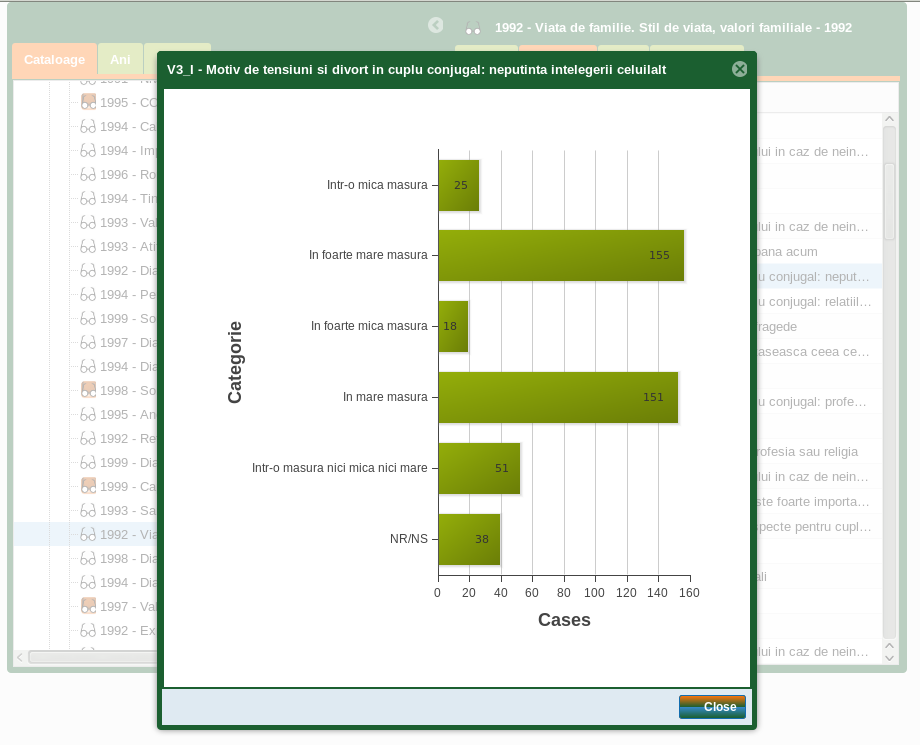
\includegraphics[width=11cm]{screenshots/details-panel-study-chart}
\par\end{centering}

\caption{Panoul care afiseaza valorile precalculate ale variabilelor}


\end{figure}


Panoul cu valori precalculate contine deocamdata graficul care afiseaza
numarul de raspunsuri la fiecare varianta pusa la dispozitie de catre
chestionar. Acest panou va fi extins pentru a contine si alte informatii,
inclusiv posibilitatea de a vedea in forma tabelara datele pe baza
carora este construit graficul. 

\begin{figure}[H]
\begin{centering}
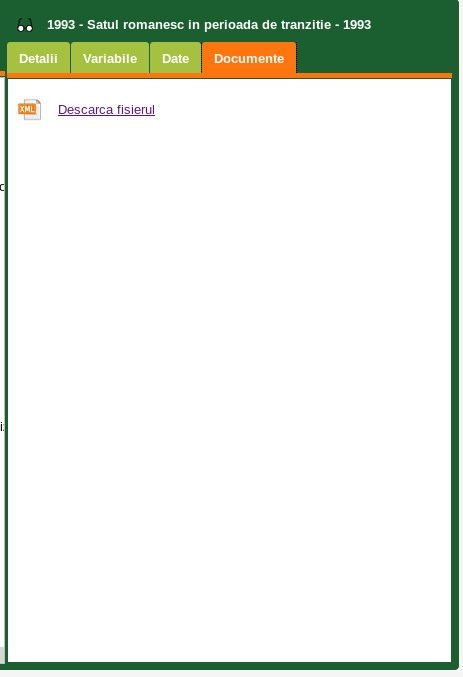
\includegraphics[width=6cm]{screenshots/details-panel-study-documente}
\par\end{centering}

\caption{Ecranul ``Studiu'', subecranul ``Documente''}


\end{figure}


Subecranul ``documente'' afiseaza si ofera spre descarcare toate
documentele atasate studiului curent. Acestea sunt dependente de modul
in care studiul a fost predat arhivei, in cazul de fata exista doar
sursa acestuia in format DDI (XML) dar in alte situatii pot exista
mult mai multe.


\subsection{Serie}

Ecranul ``Serie'' afiseaza informatii despre o serie. O serie este
un grup de studii asemanatoare, executate, de exemplu, in ani diferiti,
pentru a urmari evolutia anumitor indicatori in timp. Astfel, o serie
reprezinta pe de-o parte un demers unitar, pe de alta parte o colectie
de studii. Pentru afisarea detaliilor unei serii se folosesc doua
subecrane, unul care afiseaza metadatele seriei (titlu, rezumat, precum
si alte metadate daca sunt disponibile) si un altul care afiseaza
lista studiilor care fac parte din acea serie. 

\begin{figure}[H]
\begin{centering}
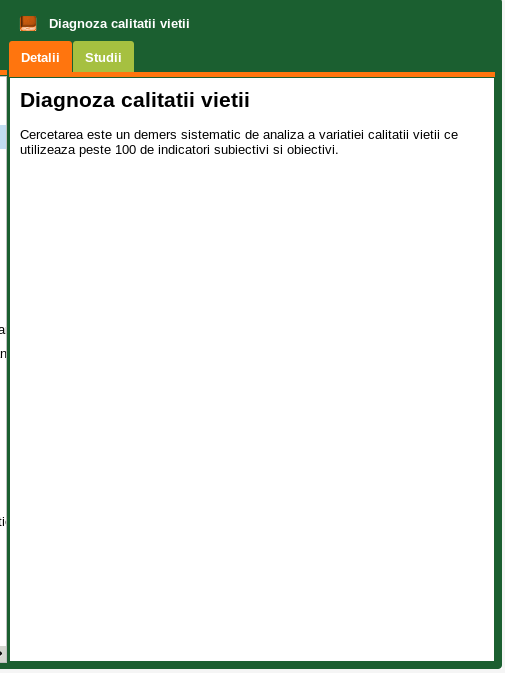
\includegraphics[width=6cm]{screenshots/details-panel-series-details}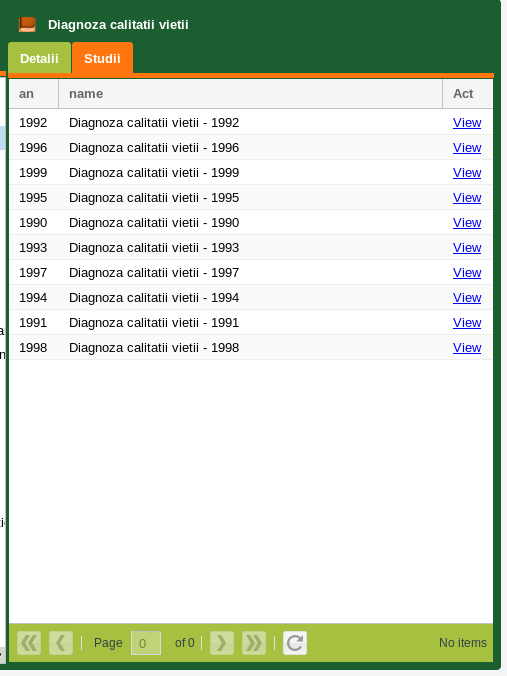
\includegraphics[width=6cm]{screenshots/details-panel-series-studies}
\par\end{centering}

\caption{Ecranul ``Serie'' subecranele ``Detalii'' si ``Studii''}


\end{figure}



\subsection{Membru al seriei}

Ecranul pentru un membru al unei serii este asemanator cu ecranul
unui studiu izolat. La el se adauga un subecran special care afiseaza
proprietatile seriei, asa cum sunt afisate si in sectiunea anterioara,
sub forma de meniu acrodeon.

\begin{figure}[H]
\begin{centering}
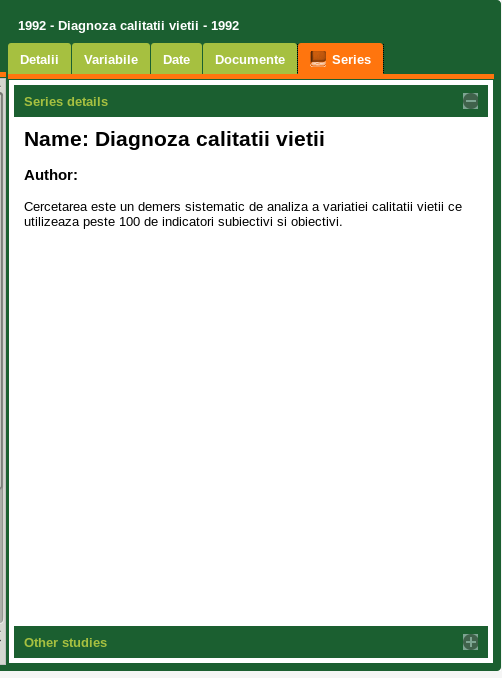
\includegraphics[width=6cm]{screenshots/details-panel-series-member-series-details}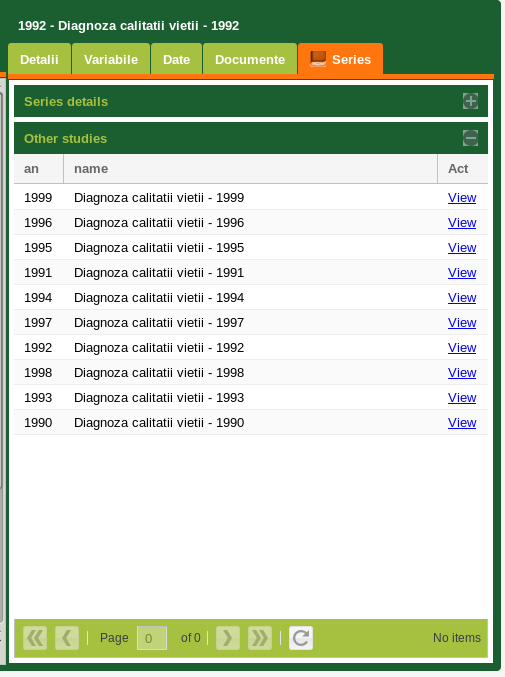
\includegraphics[width=6cm]{screenshots/details-panel-series-member-series-studies}
\par\end{centering}

\caption{Subecranul suplimentar pentru un studiu membru al unel serii}


\end{figure}

\end{document}
